\chapter{Experimento $\nu$-Angra}\label{cap:experimento}
\vspace{-2cm}

O experimento $\nu$-Angra tem como objetivo a criação de um detector de superfície capaz de detectar antineutrinos advindos da queima de combustível nuclear através da relação entre potência térmica dissipada e a taxa de eventos de antineutrinos registrados pelo detector.

O detector utiliza da radiação de Cherenkov (apêndice \ref{apdx:cherenkov}) na água para fazer a contagem de eventos. Afim de coletar os fótons gerados são utilizados 40 \ag{PMTs}, do modelo Hamamatsu R5912.



\section{O detector $\nu$-Angra}

O detector utilizado dispõe de três sistemas principais que podem ser vistos na Figura \ref{fig:detector} e serão discutidos em suas sub-sessões.

\begin{figure}[H]
    \centering
    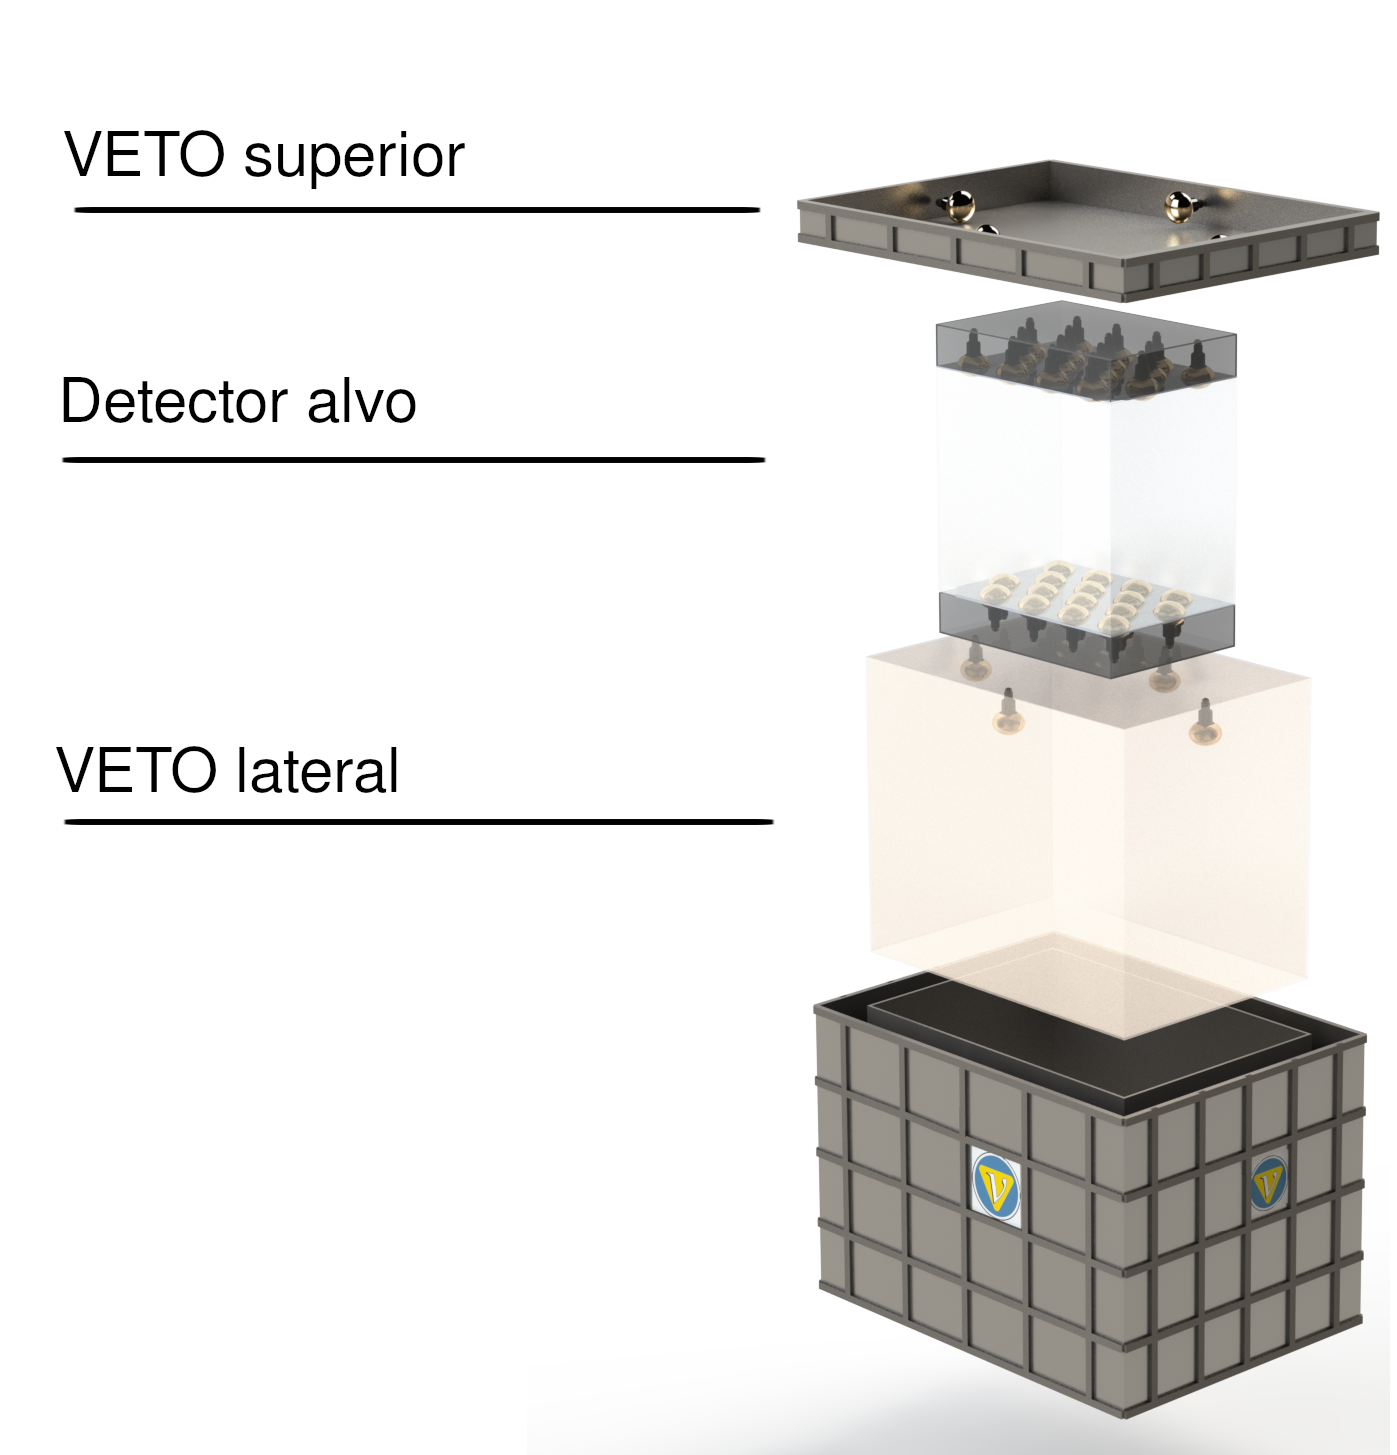
\includegraphics[width=11cm]{textuais/experimento/figuras/detector.png}
    \caption{Vista explodida do detector}
    \label{fig:detector}
\end{figure}

\subsection{Sistemas de \textit{VETO}}

Como o detector $\nu$-Angra é um detector de superfície ele não está imune à radiação advinda do cosmos, se fazendo necessário uma camada de veto para detecção de ruídos de fundo afim de selecionar apenas os eventos de antineutrinos. Cada camada de \textit{VETO} têm 4 PMTs, sendo as do \textit{VETO} superior sendo posicionadas no ponto central de cada aresta, enquanto as do \textit{VETO} lateral ficam na parte superior das faces laterais do detector, somando-se 8 PMTs 

\subsection{Detector alvo}

Como eventos de antineutrinos são de baixa energia, para melhor leitura dos eventos, o alvo apresenta 16 PMTs na sua parte inferior e 16 na parte superior, ele é preenchido com um cintilador dopado com gadolínio afim de aumentar o número de partículas livres que interagem com neutrinos através do processo de decaimento beta-inverso. O detector alvo têm volume aproximado de $1$ $m^3$

\section{Processos físicos}

\section{Reator}

\section{front-end}
